\documentclass[11pt, a4paper]{report}
\special{papersize=210mm, 297mm}
\usepackage[english]{babel}
\usepackage[utf8x]{inputenc}
\usepackage[left=2.5cm, right=2.5cm, top=2.5cm]{geometry}
\renewcommand{\baselinestretch}{1.4}
\usepackage[toc,page]{appendix}
\pagenumbering{alph}

\usepackage{amsmath}
\usepackage{graphicx}
\usepackage{float}
\graphicspath{{images/} {diagrams/}}

%\usepackage{showframe}
\usepackage{fullpage}

\usepackage{url}
%\usepackage{natbib} % for author-date citation \citep{}, \citet[]
%\usepackage{hyperref}
%\usepackage[nottoc]{tocbibind}
\usepackage{listings}
\usepackage{verbatim}
\usepackage{color}

\definecolor{dkgreen}{rgb}{0,0.6,0}
\definecolor{gray}{rgb}{0.5,0.5,0.5}
\definecolor{mauve}{rgb}{0.58,0,0.82}

\lstset{frame=tb,
	language=java,
	aboveskip=5mm, belowskip=3mm, showstringspaces=false,
	columns=flexible, basicstyle={\small\ttfamily},
	numbers=none, numberstyle=\tiny\color{gray},
	keywordstyle=\color{blue},
	commentstyle=\color{dkgreen},
	stringstyle=\color{mauve},
	breaklines=true,
	breakatwhitespace=true,
	tabsize=3
}


\usepackage{multirow}
\usepackage{array}
\newcolumntype{L}[1]{> {\raggedright\let\newline\\\arraybackslash\hspace{0pt}}m{#1}}
\newcolumntype{C}[1]{>{\centering\let\newline\\\arraybackslash\hspace{0pt}}m{#1}}
\newcolumntype{R}[1]{>{\raggedleft\let\newline\\\arraybackslash\hspace{0pt}}m{#1}}

\pagenumbering{arabic}

\begin{document}
	
	%======================================================================
	
	\begin{titlepage}
		
		\newcommand{\HRule}{\rule{\linewidth}{0.5mm}}
		
		\center
		
		\vspace{-20pt}
		
\includegraphics[width=100pt]{../images/FMI-03.png}\\[1.0cm]
		
		\textsc{\LARGE West University of  Timisoara}\\[0.5cm]
		\textsc{\Large Faculty of Mathematics and Computer Science}\\[0.5cm]
		\textsc{\large Study Program: \\Computer Science in English}\\[3cm]
		\textsc{\Huge Master Dissertation}\\[5cm]
		
		\begin{minipage}{0.4\textwidth}
			\begin{flushleft} \large
				\textbf{COORDINATOR:}\\
				Associate Prof. Marc Eduard \textsc{Frîncu}
			\end{flushleft}
		\end{minipage}
		~
		\begin{minipage}{0.4\textwidth}
			\begin{flushright} \large
				\textbf{GRADUATE:} \\
				Maria Minerva \textsc{Vonica}
			\end{flushright}
		\end{minipage}\\[0.5cm]
			
		\vfill
		{\large Timi\c{s}oara \\2021}\\
		\vfill
		
	\end{titlepage}
	
	% =====================================================================
	
	\begin{titlepage}
		
		\newcommand{\HRule}{\rule{\linewidth}{0.5mm}}
		
		\center
		
		\textsc{}\\[.7cm]
		
		\textsc{\LARGE West University of  Timi\c{s}oara}\\[0.5cm]
		\textsc{\Large Faculty of Mathematics and Computer Science}\\[0.5cm]
		\textsc{\large Study Program: \\Computer Science in English}\\[4.5cm]
		
		\textsc{\Huge Master Dissertation}\\[2cm]
		
		{\Huge \bfseries Name}\\[6cm]
		
		\begin{minipage}{0.4\textwidth}
			\begin{flushleft} \large
				\textbf{COORDINATOR:}\\
				Associate Prof. Marc Eduard \textsc{Frîncu}
			\end{flushleft}
		\end{minipage}
		~
		\begin{minipage}{0.4\textwidth}
			\begin{flushright} \large
				\textbf{GRADUATE:} \\
				Maria-Minerva \textsc{Vonica}
			\end{flushright}
		\end{minipage}\\[0.5cm]
		\vfill
		{\large Timi\c{s}oara\\ 2021}\\
		
		\vfill
		
	\end{titlepage}

	% =====================================================================
	
	\chapter{Application}
	\section{Dataset}
	In order to build the dataset, we made use of the freely available data from the Landsat Archive, specifically from collection 1, level 1. This consists of data products generated from Landsat 8 Operational Land Imager/Thermal Infrared Sensor, Landsat 7 Enhanced Thematic Mapper Plus, Landsat 4-5 Thematic Mapper, and Landsat 1-5 Multispectral Scanner instruments \cite{C1L1}. For the purpose of this paper, we will focus only on images collected from the Landsat 8 satellite.
	
	\subsection{Landsat 8}

	For the purpose of this paper, we will use images collected by the Landsat 8 satellite (Figure 1.1), which was launched on an Atlas-V rocket from Vandenberg Air Force Base, California on February 11, 2013. Landsat 8 is the most recently launched Landsat satellite and carries the Operational Land Imager (OLI) and the Thermal Infrared Sensor (TIRS) instruments.
	
	\begin{figure}[h]
		\centering
		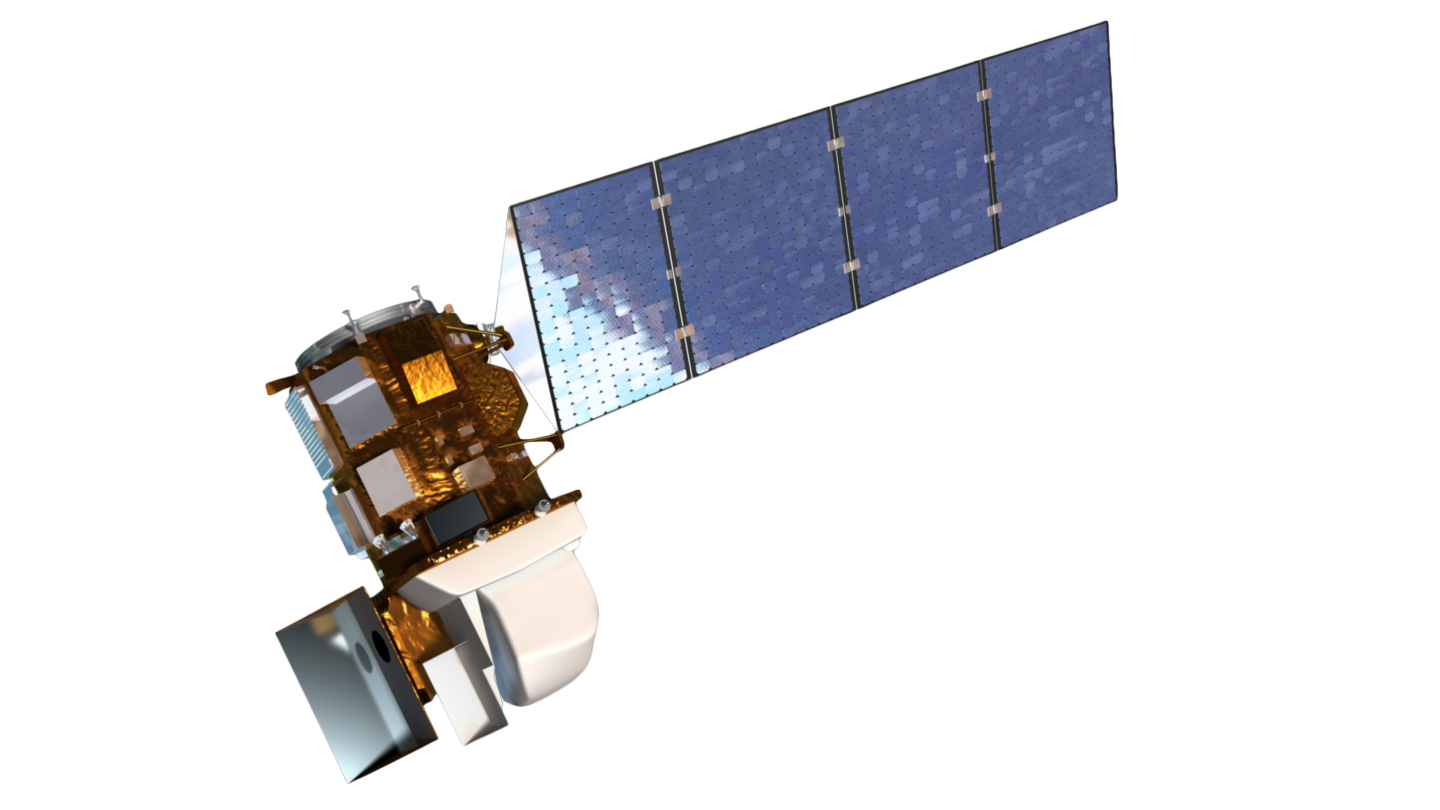
\includegraphics[scale=0.25]{../images/LandsatSatellite.png}
		\caption{LandsatSatellite \cite{LANDSATPIC}}
		\label{fig:LandsatSatellite}
	\end{figure}
	
	Landsat 8 orbits the Earth in a sun-synchronous, near-polar orbit, at an altitude of 705 km, inclined at 98.2 degrees, and completes one Earth orbit every 99 minutes.  The satellite has a 16-day repeat cycle with an equatorial crossing time: 10:00 a.m. +/- 15 minutes. It acquires about 740 scenes a day on the Worldwide Reference System-2 (WRS-2) path/row system, with a swath overlap (or sidelap) varying from 7\% at the equator to a maximum of approximately 85\% at extreme latitudes. A Landsat 8 scene size is 185 km x 180 km \cite{LANDSAT}.
	
	\subsubsection{Operational Land Imager}
	
	The Operational Land Imager (OLI) is a remote sensing instrument aboard Landsat 8, built by Ball Aerospace \& Technologies. The sensor collects moderate resolution data that is used to monitor changing trends on the surface and evaluate how land usage changes over time. The images and data that OLI has helped collect have practical applications today in agriculture, mapping, and monitoring changes in snow, ice, and water \cite{lolidcp}. 

	The OLI operates in the visible (VIS) and short wave infrared (SWIR) spectral region, having a width of 185 km. It uses nine channels, which range from wavelengths of 443 nm to 2,200 nm. Of these nine channels, eight are multispectral and one is panchromatic. The eight multispectral channels have a 30-meter spatial resolution, and the panchromatic channel has a 15 meters one.
	
	\subsubsection{Thermal Infrared Sensor}
	
	The Thermal Infrared Sensor (TIRS) measures land surface temperature in two thermal bands with a new technology that uses Quantum Well Infrared Photodetectors to detect long wavelengths of light emitted by the Earth whose intensity depends on surface temperature. These wavelengths, called thermal infrared, are well beyond the range of human vision \cite{tirs}.
	
	\subsubsection{OLI and TIRS bands}
	
	Landsat 8 acquires data from these sensors in in 11 bands, as following in table \ref{table:bands_table}.
	
	\begin{table} [h]
		\center
		\begin{tabular} {|  l | l | l |}
			\hline
			\textbf{Bands} & \textbf{Wavelength (micrometers)} & \textbf{Resolution (meters)} \\ [0.2ex]
			\hline
			Band 1 - Coastal aerosol & 0.43-0.45 & 30 \\ [0.2ex]
			\hline
			Band 2 - Blue & 0.45-0.51 & 30 \\ [0.2ex]
			\hline
			Band 3 - Green & 0.53-0.59 & 30 \\ [0.2ex]
			\hline
			Band 4 - Red & 0.64-0.67 & 30 \\ [0.2ex]
			\hline
			Band 5 - Near Infrared (NIR) & 0.85-0.88 & 30 \\ [0.2ex]
			\hline
			Band 6 - SWIR 1 & 1.57-1.65 & 30 \\ [0.2ex]
			\hline
			Band 7 - SWIR 2 & 2.11-2.29 & 30 \\ [0.2ex]
			\hline
			Band 8 - Panchromatic & 0.50-0.68 & 15 \\ [0.2ex]
			\hline
			Band 9 - Cirrus & 1.36-1.38 & 30 \\ [0.2ex]
			\hline
			Band 10 - Thermal Infrared (TIRS) 1 & 10.6-11.19 & 100 \\ [0.2ex]
			\hline
			Band 11 - Thermal Infrared (TIRS) 2 & 11.50-12.51 & 100 \\ [0.2ex]
			\hline
		\end{tabular}
		\caption{Landsat 8-9 Operational Land Imager (OLI) and Thermal Infrared Sensor (TIRS) bands \cite{bands}.}
		\label{table:bands_table}
	\end{table}
	
	\subsection{World Glacier Inventory}
	The World Glacier Inventory (WGI) proves to be a useful resource for building our dataset, since it contains information for over 130,000 glaciers. Inventory parameters include geographic location, area, length, orientation, elevation, and classification. The WGI is based primarily on aerial photographs and maps with most glaciers having one data entry only. Hence, the data set can be viewed as a snapshot of the glacier distribution in the second half of the 20th century. It is based on the original WGI (WGMS 1989) from the World Glacier Monitoring Service \cite{WGI}.  
	
	There are a number of ways to retrieve data from the inventory:
	\begin{itemize}
		\item download the entire database in a single ASCII text file (wgi\_feb2012.csv);
		\item search by parameter using the Search Inventory interface;
		\item extract regions through the Extract Selected Regions interface.
	\end{itemize}

	The ASCII text file will be used with the purpose to define which are the glaciers to be included in the dataset to be built. An example of how this file looks like can be found in Figure 1.1.
	
	\begin{figure}[h]
		\centering
		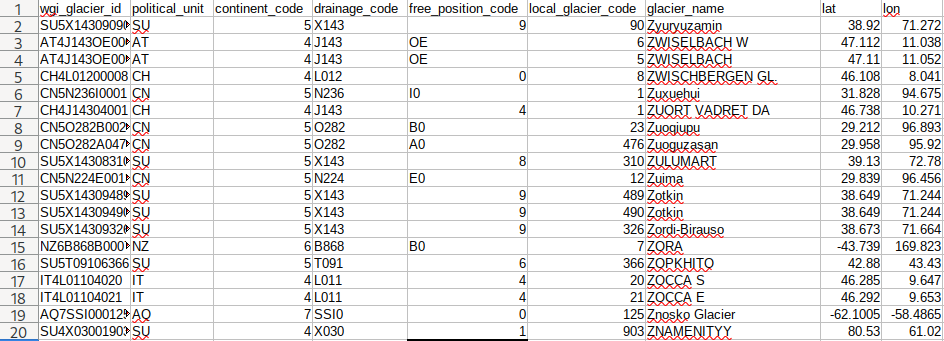
\includegraphics[scale=0.5]{../images/wgi_ASCII_file.png}
		\caption{WGI ASCII}
		\label{fig:WGI_ASCII}
	\end{figure}
	
	The \emph{parameters} which will be extracted for the dataset construction are the following:
	\begin{itemize}
		\item \textit{wgi\_glacier\_id}: unique id representing one glacier (or part of it, if the coverage area is larger);
		\item \textit{glacier\_name}: name of the glacier (if it has one);
		\item \textit{lat}: latitude of the glacier;
		\item \textit{lon}: longitude of the glacier.
	\end{itemize}

	\subsection{Asset Acquisition}	
	
	Since Landsat 8 acquires over 700 scenes per day, this means that there are over two million scenes available for download, either making use of already built user friendly tools or by simply querying for them directly.
	
	\subsubsection{USGS Earth Explorer}
	
	One of the most popular services for satellite imagery downloading is USGS Earth Explorer. This is used for querying and ordering of satellite images, aerial photographs, and cartographic products through the U.S. Geological Survey. The tool is particularly useful when the main focus is to analyse a specific area rather than trying to acquire a large dataset of scenes. One can easily search for assets based on criteria such as world reference system path and row variables, latitude, longitude, cloud coverage, capture date and many others \cite{USGS}.
	
	However, downloading a large set of assets proves to be rather difficult by using this tool alone, since the parameters for each scene need to be manually set. On top of this, the query results have to be picked by hand and then passed for downloading through another application which handles their bulk download. This makes the process of building the dataset rather slow, frustrating and error prone. Such an example can be viewed in Figure 1.2, for the Belvedere glacier (45.9830, 6.888).
	
	\begin{figure}[h]
		\centering
		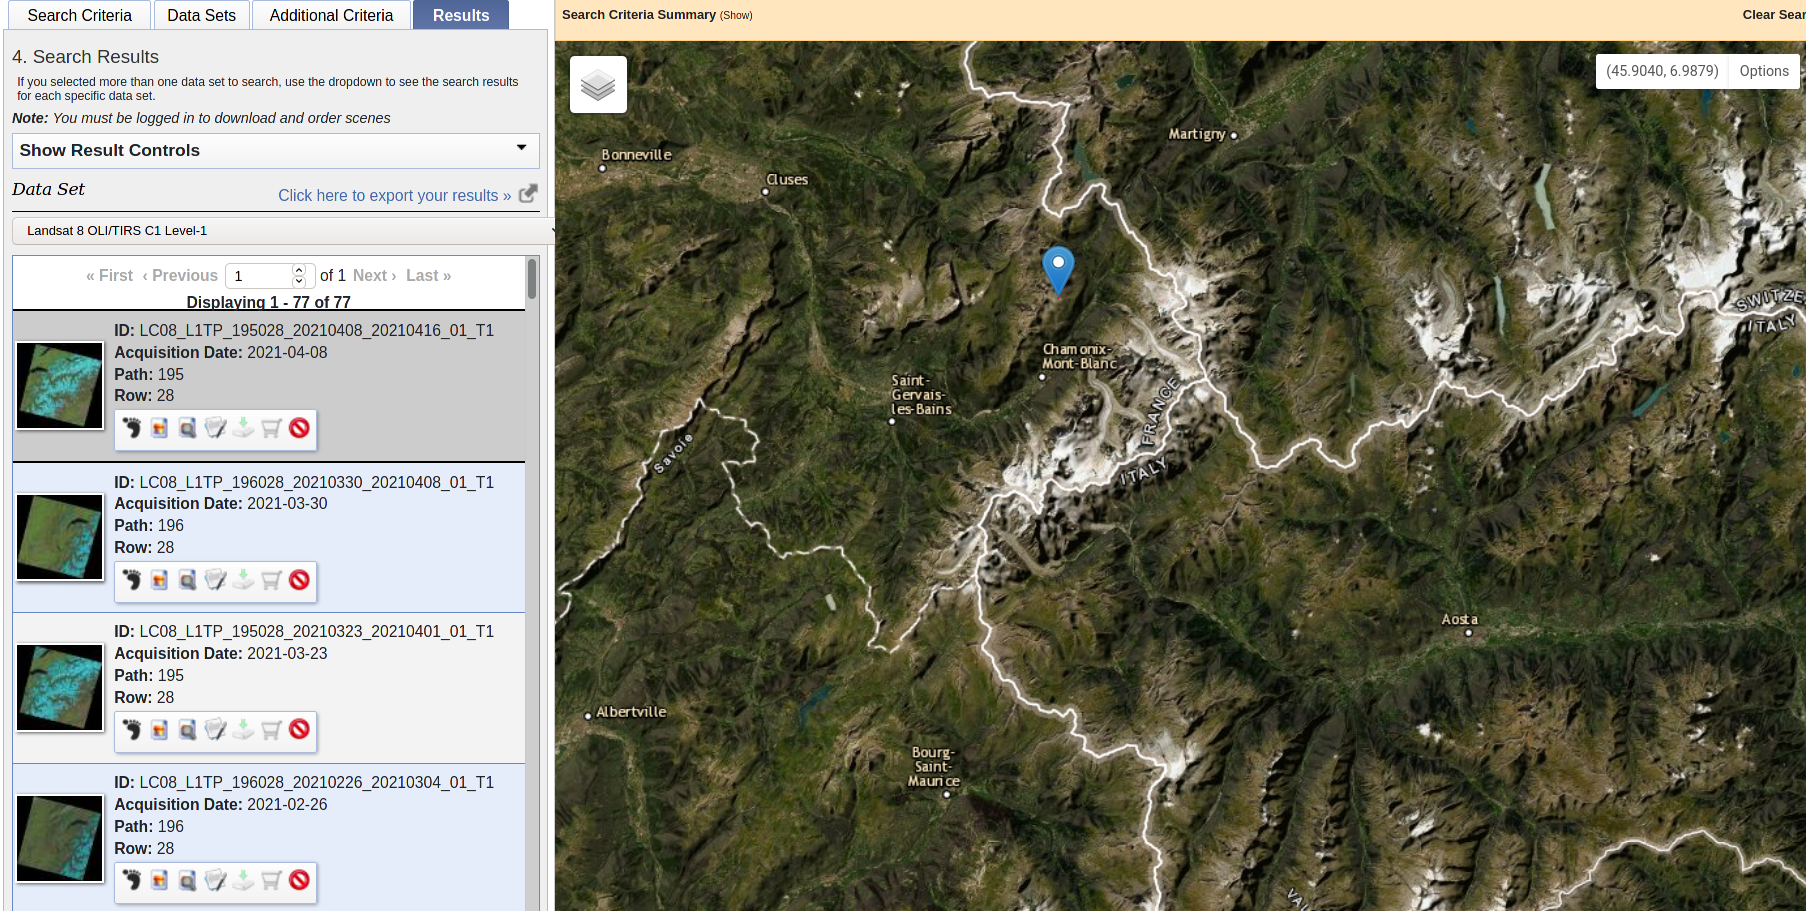
\includegraphics[scale=0.25]{../images/EarthExplorer.png}
		\caption{EarthExplorer}
		\label{fig:EarthExplorer}
	\end{figure}
	
	\subsubsection{SpatioTemporal Asset Catalog API}
	
	In order to fix the problem of excessive manual labour which appeared by using the USGS Earth Explorer, we rather implemented an endpoint of the SpatioTemporal Asset Catalog API, specifically, the following: \textbf{\url{http://nsidc.org/data/glacier_inventory/index.html}} \cite{STAC}. The main idea of searching by using parameters still remains, but instead of manual inputting data for the search data, we rely on using the above-mentioned World Glacier Inventory ASCII text file, since it already has all the required information for each glacier.
	
	By using this method we can pick which glaciers we want to download based on their coordinates and calculate a bounding box representing the area we want to search, required for the STAC API query. Since there might be clouds which could obfuscate the area of interest in the image, we also add a maximum allowed cloud coverage along the bounding box.
	
	The STAC API query also requires a name for the collection of assets we want our queries to be made on, which for us is landsat-8-l1 (Landsat 8 Collection 1, Level 1). Using these three parameters we can now easily acquire a large number of assets with minimal manual labour, as compared to the more user friendly tool provided by USGS.
	
	The downloaded assets will be stored at a user specified disk location and they will be structured as shown in the Figure 1.3.
	
	\begin{figure}[h]
		\centering
		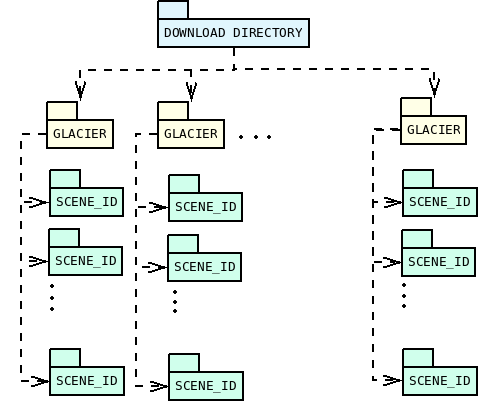
\includegraphics[scale=0.55]{../images/DownloadDirectory.png}
		\caption{Download Directory}
		\label{fig:DownloadDirectory}
	\end{figure}

	\section{Crawling}
	\section{NDSI}

	\chapter{Implementation}
	\section{Download}
	
	
	\tableofcontents{}
	\addcontentsline{toc}{chapter}{List Of Figures}
	\listoffigures{}
	\addcontentsline{toc}{chapter}{List Of Tables}
	\listoftables{}
	
	\bibliographystyle{alpha}
	\bibliography{references}
		
	\chapter{Glossary}
	
	% ==================================================================
	
	\section{Acronyms}
	
		\begin{table} [H]
		\centering
		\begin{tabular} {|  l | L{10cm} |}
			\hline
			WGI & World Glacier Inventory \\ [0.2ex]
			\hline
		\end{tabular}
		\caption{Acronyms table }
		\label{table:acron}
	\end{table}
	\end{document}
